\section{Interferometric stabilisation of reservoir cavity}

\begin{frame}{Classical cavity stabilisation}
	\begin{columns}
		\begin{column}{.5\textwidth}
			\begin{figure}
				\centering
				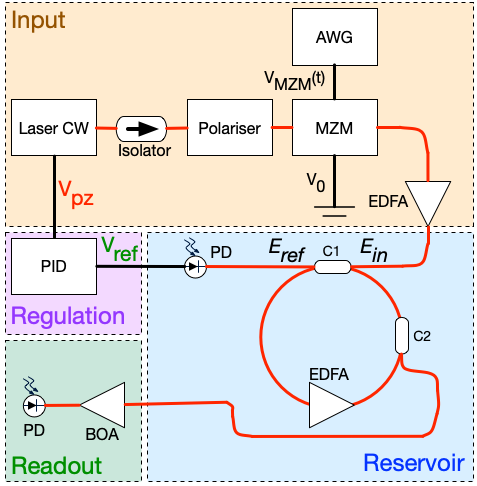
\includegraphics[width=\textwidth]{exp-setup3.png}
			\end{figure}
		\end{column}%
		\begin{column}{.5\textwidth}
			\begin{figure}
				\centering
				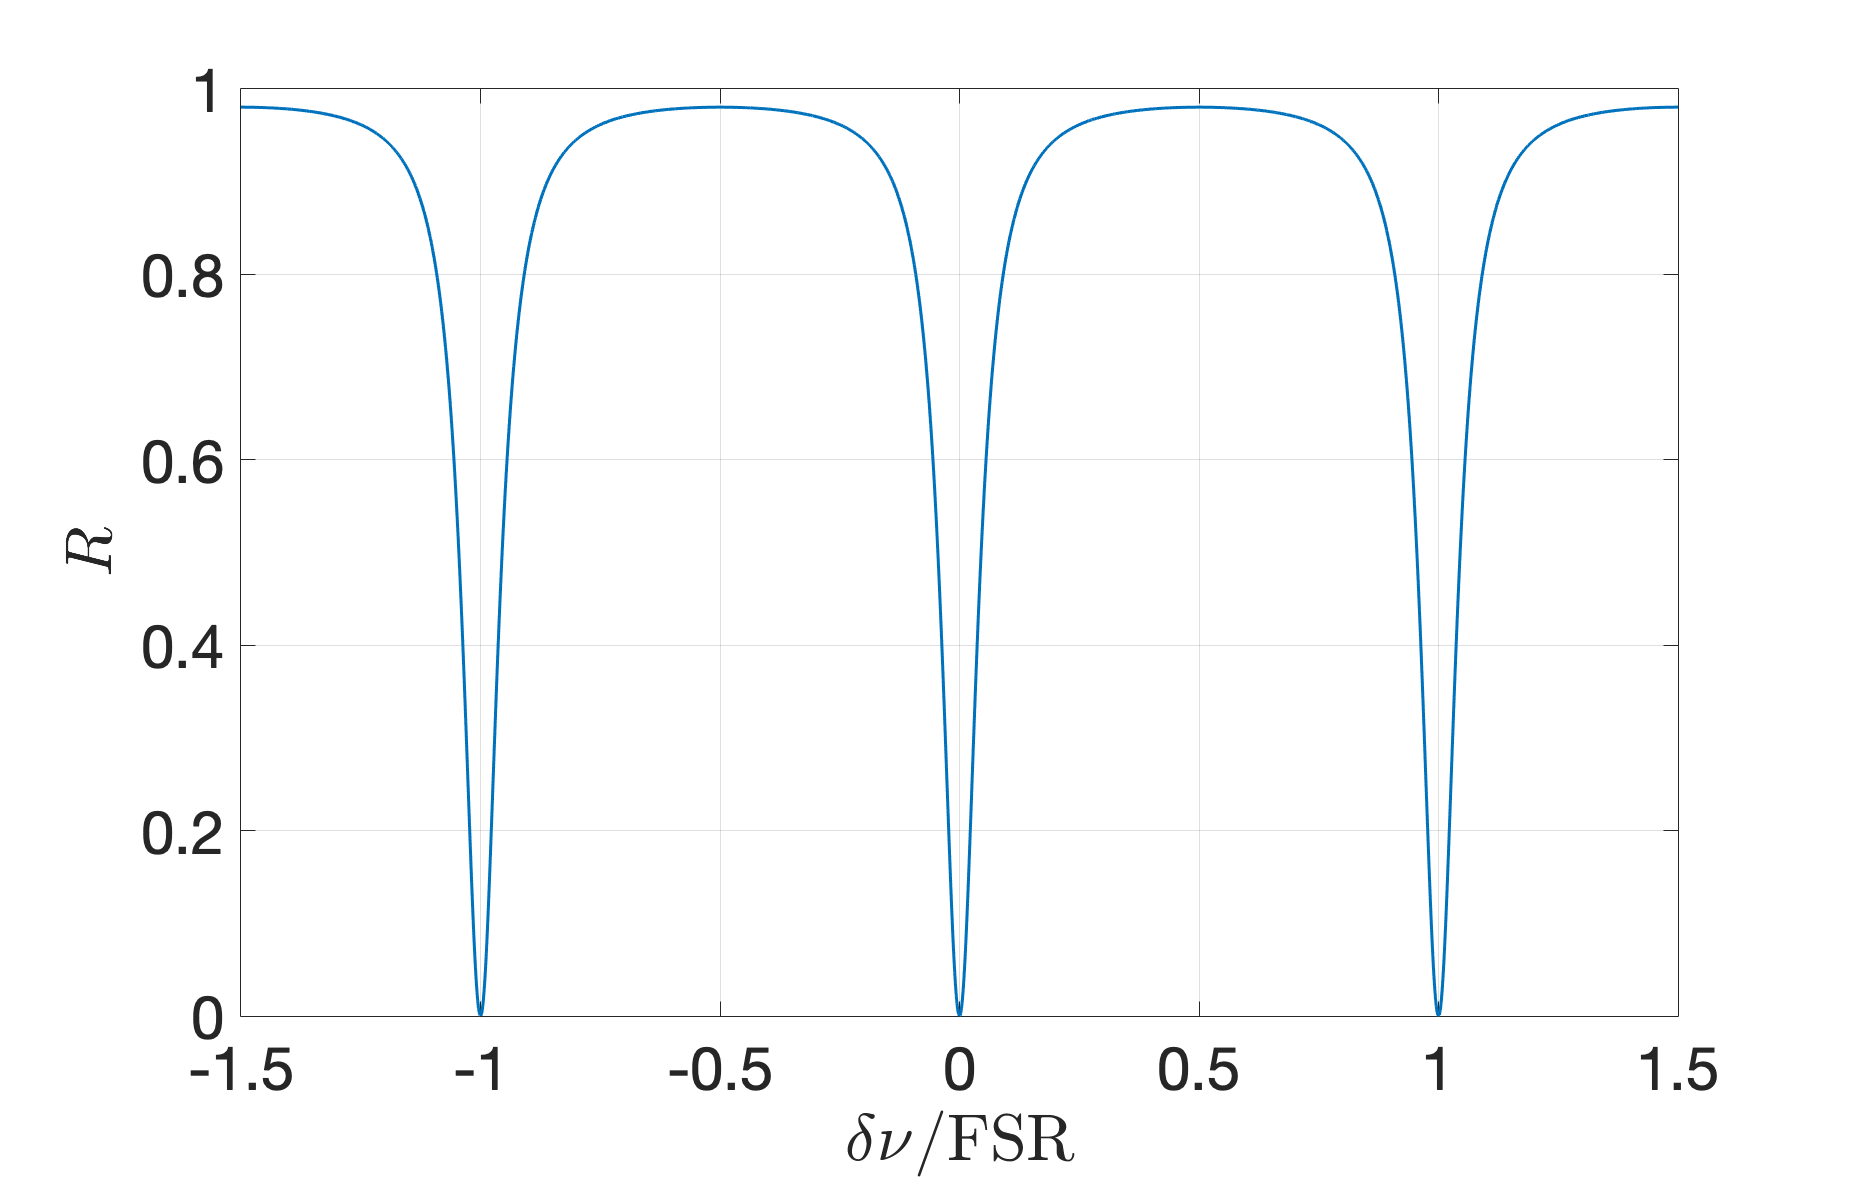
\includegraphics[width=\textwidth]{fp-ref-tf.png}
			\end{figure}
			\begin{itemize}
				\item Stabilisation of $\color{ForestGreen} V_{\text{ref}}$ using $\color{red} V_{\text{pz}}$
				\item Limitation : \textbf{symmetry}
			\end{itemize}
		\end{column}
	\end{columns}
\end{frame}

\begin{frame}{Pound-Drever-Hall technique}
	\begin{columns}
		\begin{column}{.5\textwidth}
			\begin{figure}
				\centering
				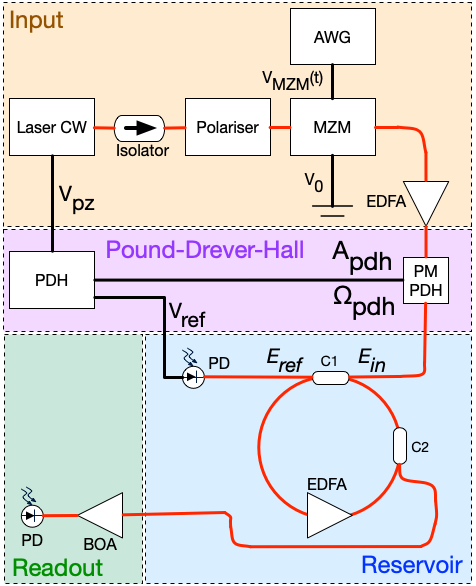
\includegraphics[width=\textwidth]{exp-setup4.png}
			\end{figure}
		\end{column}%
		\begin{column}{.5\textwidth}
			\begin{figure}
				\centering
				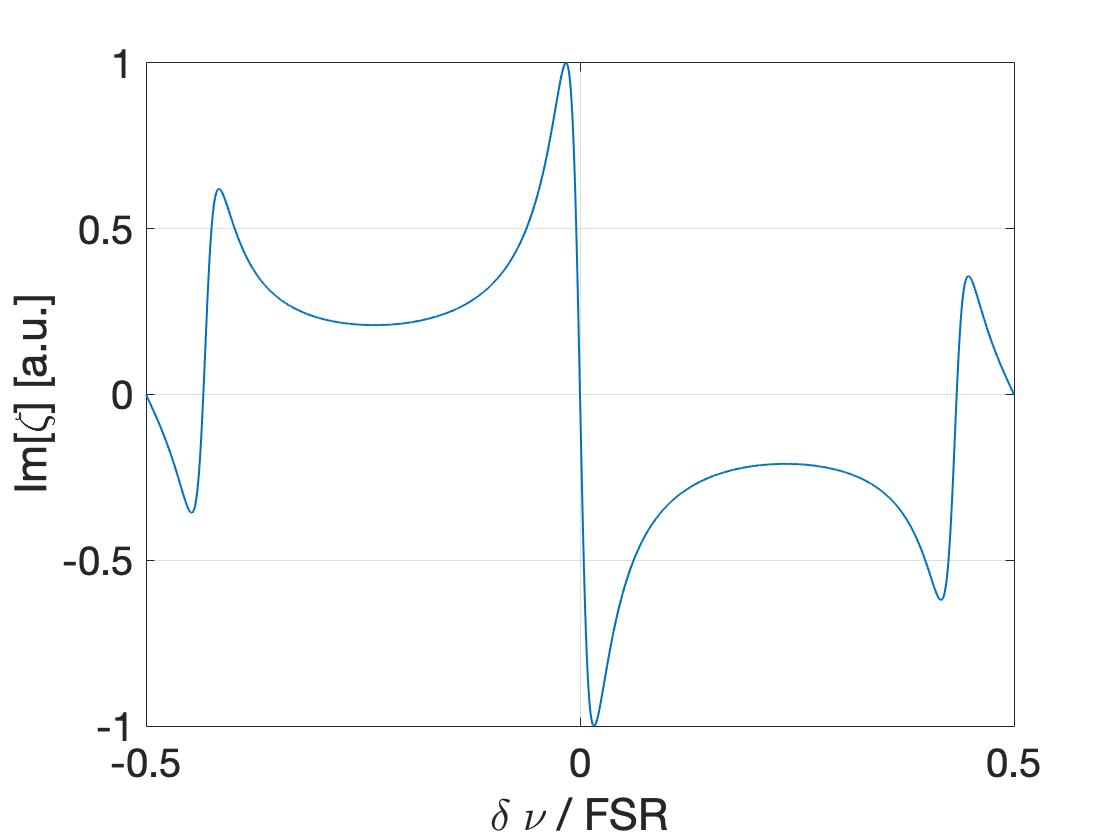
\includegraphics[width=\textwidth]{im_zeta.png}
			\end{figure}
			\begin{itemize}
				\item Phase modulation + lock-in amplification
				\item Error function \textbf{anti-symmetric}
			\end{itemize}
			\centering
			$\color{red}\hookrightarrow$ \alert{Better performances !}
		\end{column}
	\end{columns}
\end{frame}

\begin{frame}{PDH technique for reservoir cavity \textbf{with} phase modulation}
	\begin{columns}
		\begin{column}{.5\textwidth}
			\begin{figure}
				\centering
				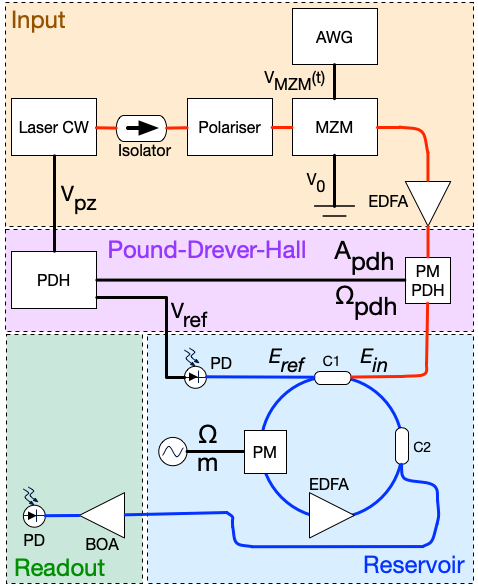
\includegraphics[width=\textwidth]{exp-setup5.png}
			\end{figure}
		\end{column}%
		\begin{column}{.5\textwidth}
			\begin{figure}
				\centering
				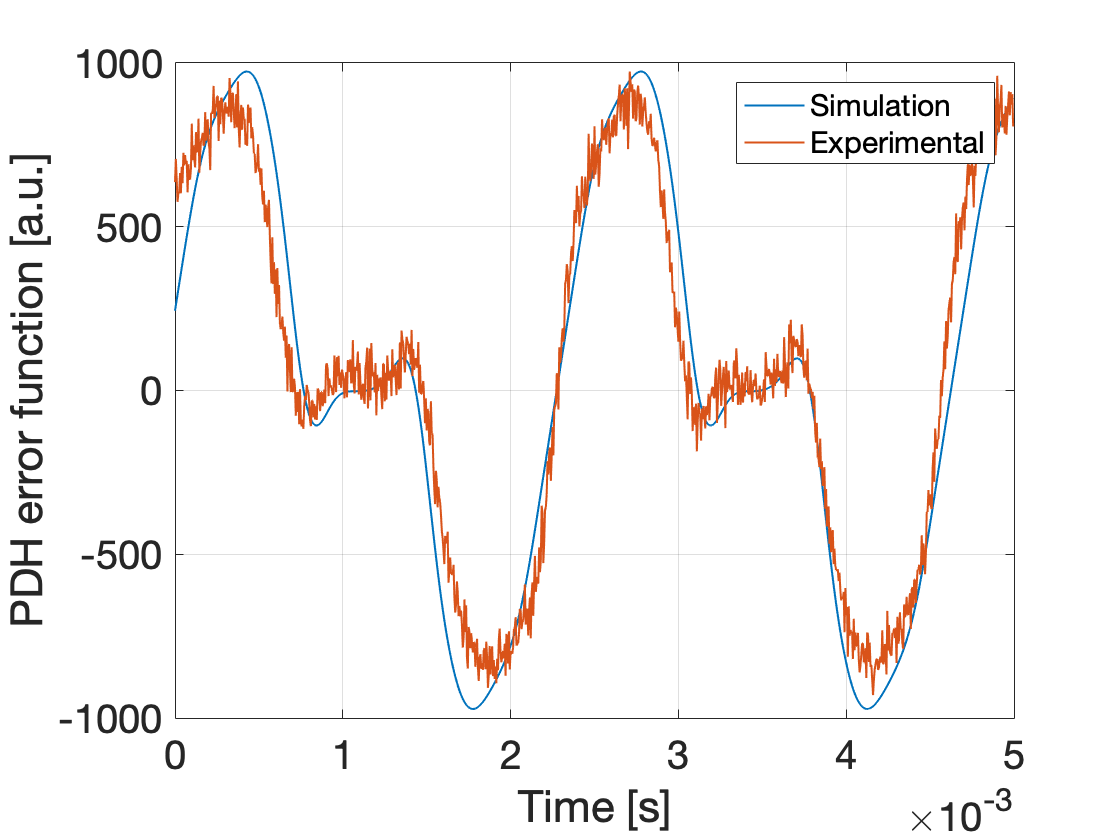
\includegraphics[width=\textwidth]{3130_4.png}
			\end{figure}
			\begin{itemize}
				\item Linear regions with steep slopes
			\end{itemize}
			\centering
			$\color{red}\hookrightarrow$ \alert{PDH error signal can be used !}
		\end{column}
	\end{columns}
\end{frame}

\begin{frame}{Cavity stabilisation performances}
	\begin{itemize}
		\item PDH parameters to explore
		\item Reservoir computer performances degraded by \textbf{phase noise} and \textbf{modulation amplitude} $\Rightarrow$ \alert{tradeoff !}
		\item Figure of merit : $\text{Challenger} = \sigma_{\text{PDH}} \cdot \Delta \varphi$
	\end{itemize}
	\centering
	$\hookrightarrow$ Should be minimised !
\end{frame}

\begin{frame}{Results}

	\begin{table}
		\centering
			\begin{tabular}{|c|c|c|c|c|c|}
				\hline
				\small{Rank} & $A_{\text{PDH}}$ [\si{\voltptp}] & $\nu_{\text{PDH}}$ [\si{\kilo\hertz}] & $\epsilon^*$ [\si{\au}] & $\phi$ [\si{\radian}] & \small{Challenger} [\si{\milli\radian\squared}]\\
				\hline
				\hline
				\#1 & 0.4 & 781 & 400 & 1.3 & 292\\
				\#2 & 0.2 & 781 & -300 & -1.43 & 327\\
				\#3 & 0.4 & 781 & 700 & 1.45 & 337\\
				\#4 & 0.3 & 781 & 500 & 1.31 & 362\\
				\#5 & 0.4 & 781 & 600 & 1.39 & 377\\
				\hline
			\end{tabular}
	\end{table}
	
	\begin{itemize}
		\item Best modulation frequency $\nu_{\text{PDH}} = \SI{781}{\kilo\hertz}$
		\item However, measurements not very reproducible so far...
		\item Not possible to use the cavity as a reservoir computer\\ $\Rightarrow$ \textbf{still too much noise}
	\end{itemize}
	
\end{frame}